\documentclass{beamer}

\usepackage[utf8]{inputenc}
\usepackage{csquotes}
\usepackage{latexsym,amsmath,xcolor,multicol,booktabs,calligra, animate, subfig}
\usepackage{graphicx,pstricks,listings,stackengine, bbm}
\usepackage{tikz}
\usetikzlibrary{fit,tikzmark}   
\usepackage{booktabs,cellspace}
\usepackage{color, colortbl}
\usepackage{hyperref}
\usepackage{color}
%Information to be included in the title page:
\title{Designing Equitable Electricity Systems}
\author{Lauren Beatty\\ \href{mailto:lbeatty@edf.org}{lbeatty@edf.org}\\
\vspace{.5cm}\\
Matthias Fripp\\
\href{mailto:mfripp@edf.org}{mfripp@edf.org}}
\institute{Environmental Defense Fund}
\date{May 6, 2024}


%% Tikz
\usepackage{tikz}
\usetikzlibrary{shapes.geometric, arrows}

\tikzstyle{start} = [rectangle, rounded corners, 
minimum width=3cm, 
minimum height=1cm,
text centered, 
draw=black, 
fill=orange!30]

\tikzstyle{process} = [rectangle, 
minimum width=3cm, 
minimum height=1cm, 
text centered, 
text width=3cm, 
draw=black, 
fill=blue!30]

\tikzstyle{stop} = [rectangle, rounded corners, 
minimum width=3cm, 
minimum height=1cm,
text centered, 
draw=black, 
fill=green!30]

\tikzstyle{arrow} = [thick,->,>=stealth]


\logo{
\includegraphics[height=1cm]{EDF_color_webRGB_2022 (2).png}\hspace*{.03\paperwidth}\vspace{.01\paperwidth}}


%Color Pallete
\definecolor{EDFblue}{RGB}{0.0, 51, 204}
\definecolor{EDFgreen}{RGB}{0, 153, 51} 
\definecolor{EDFlightgreen}{RGB}{161, 226, 20}
\definecolor{EDFcyan}{RGB}{51,204,255}
\setbeamercolor{structure}{fg=EDFblue} 
\setbeamercolor{button}{bg=EDFblue,fg=white}
\setbeamertemplate{navigation symbols}{}
\newcommand{\nologo}{\setbeamertemplate{logo}{}} % command to set the logo to nothing


\hypersetup{colorlinks,linkcolor=EDFblue,urlcolor=EDFblue}


\begin{document}

\frame{\titlepage}

\begin{frame}
\frametitle{Introduction}
\textbf{Main Question:  How do we design electrical systems that center equity and justice \textit{without} sacrificing efficiency?}
\vspace{1cm}

\paragraph{\textbf{Previous Paradigm}}
\begin{itemize}
    \item Potentially harmful and polluting infrastructure is sited disproportionately near poor and marginalized communities.
    \item Planning decisions are informed by \textit{least cost} models.
    \item Communities are left in the lurch by technological changes.
\end{itemize}
\end{frame}

\begin{frame}{Background on Least-Cost Electricity Planning Models}
\begin{center}
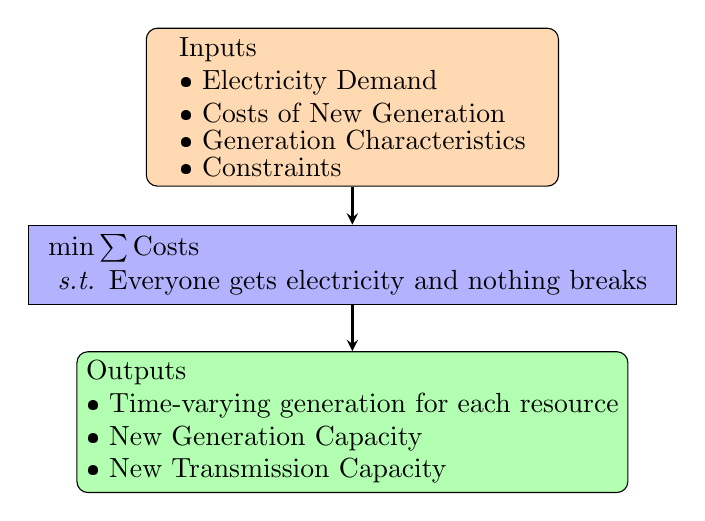
\begin{tikzpicture}[node distance=2cm]
\node (start) [start, text width=5cm] {\shortstack[l]{Inputs\\• Electricity Demand \\ • Costs of New Generation \\ • Generation Characteristics\\
• Constraints}};

\node(obj)[process, below of=start, text width=8cm]{\shortstack[l]{$\min \sum \text{Costs}$ \\ \textit{ 
   s.t.   }\text{Everyone gets electricity and nothing breaks }}};

\node (result) [stop, below of=obj] {\shortstack[l]{Outputs\\• Time-varying generation for each resource \\ • New Generation Capacity \\ • New Transmission Capacity}};

\draw [arrow] (start) -- (obj);
\draw [arrow] (obj) -- (result);

\end{tikzpicture}
\end{center}
\end{frame}

{\nologo
\begin{frame}{Previous Attempts to Shoehorn Justice Into these Models}
\begin{center}
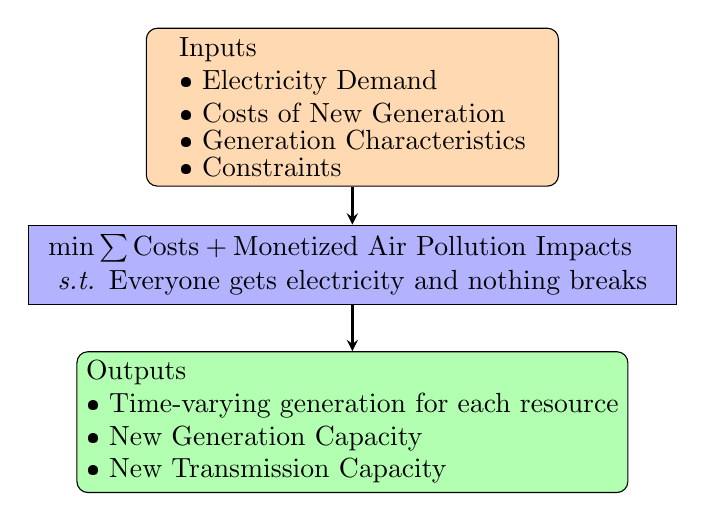
\begin{tikzpicture}[node distance=2cm]

\node (start) [start, text width=5cm] {\shortstack[l]{Inputs\\• Electricity Demand \\ • Costs of New Generation \\ • Generation Characteristics\\
• Constraints}};

\node(obj)[process, below of=start, text width=8cm]{\shortstack[l]{$\min \sum \text{Costs} + \text{Monetized Air Pollution Impacts}$ \\ \textit{ 
   s.t.   }\text{Everyone gets electricity and nothing breaks }}};

\node (result) [stop, below of=obj] {\shortstack[l]{Outputs\\• Time-varying generation for each resource \\ • New Generation Capacity \\ • New Transmission Capacity}};

\draw [arrow] (start) -- (obj);
\draw [arrow] (obj) -- (result);

\end{tikzpicture}
\end{center}

\begin{itemize}
    \item Monetized impacts don't consider unjust distributional consequences.
    \item Equity weights can be difficult to generate and defend.
\end{itemize}

\end{frame}}

{\nologo
\begin{frame}{Our Approach}
    \begin{center}
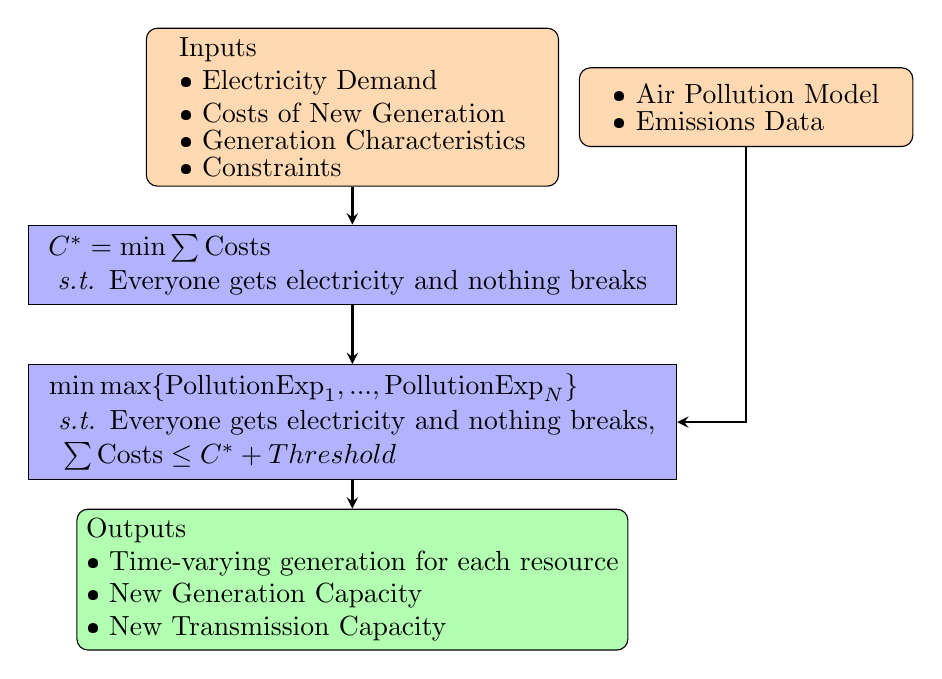
\begin{tikzpicture}[node distance=2cm]

\node (start) [start, text width=5cm] {\shortstack[l]{Inputs\\• Electricity Demand \\ • Costs of New Generation \\ • Generation Characteristics\\
• Constraints}};

\node (air) [start, text width=4cm, right of= start, xshift=3cm] {\shortstack[l]{• Air Pollution Model\\
• Emissions Data}};

\node(obj)[process, below of=start, text width=8cm, xshift=0cm]{\shortstack[l]{$C^* = \min \sum \text{Costs}$ \\ \textit{ 
   s.t.   }\text{Everyone gets electricity and nothing breaks }}};

\node(obj2)[process, below of=obj, text width=8cm, xshift=0cm]{\shortstack[l]{$\min \max\{\text{PollutionExp}_1,...,\text{PollutionExp}_N\}$ \\ \textit{ 
   s.t.   }\text{Everyone gets electricity and nothing breaks,} \\
    $\text{      }\sum \text{Costs} \leq C^*+Threshold$ }};

\node (result) [stop, below of=obj2] {\shortstack[l]{Outputs\\• Time-varying generation for each resource \\ • New Generation Capacity \\ • New Transmission Capacity}};

\draw [arrow] (start) -- (obj);
\draw [arrow] (air) |- (obj2);
\draw [arrow] (obj) -- (obj2);
\draw [arrow] (obj2) -- (result);


\end{tikzpicture}
\end{center}
\end{frame}}


\begin{frame}{Our Approach}
    \begin{enumerate}
        \item Use EPA emissions data to calculate emissions rates (Pounds per MWh)
        \item Use InMap Source-Receptor Matrix to calculate how one MWh of generation for each resource affects population-weighted average exposure for different groups.
        \item Use Switch to calculate least cost planning costs.
        \item Modify and run Switch to minimize air pollution exposure subject to a cost constraint.
    \end{enumerate}

\paragraph{Benefits}
\begin{itemize}
    \item Avoids the use of equity weights while still centering distributional concerns.
    \item Still finds low-cost solutions.
    \item Generalizable framework
\end{itemize}
\end{frame}


\begin{frame}{A Point About Calculus}
    
\includegraphics[width=0.48\textwidth]{Figures/Slide Pictures/Transmission1.png} 
\includegraphics[width=0.48\textwidth]{Figures/Slide Pictures/Transmission2.png}

    The effect of deviations from the least-cost optimum will depend on the shape of the objective function.  This is an \textit{empirical} question!\\
    \vspace{.5cm}
    $\Rightarrow$ Perhaps you can get large improvements in health or jobs at only modest increases in cost.
\end{frame}

\begin{frame}{Thanks!}
\label{Thanks}


    Please feel free to contact me at:
    \href{mailto:lbeatty@edf.org}{lbeatty@edf.org}\\
    \vspace{1cm}
\end{frame}

\begin{frame}{Bonus Slide!}
    This project started as a side-project to the Model Intercomparison Project -- a project aimed at harmonizing the inputs and comparing multiple open-source electricity planning models.

    \vspace{.4cm}
    
    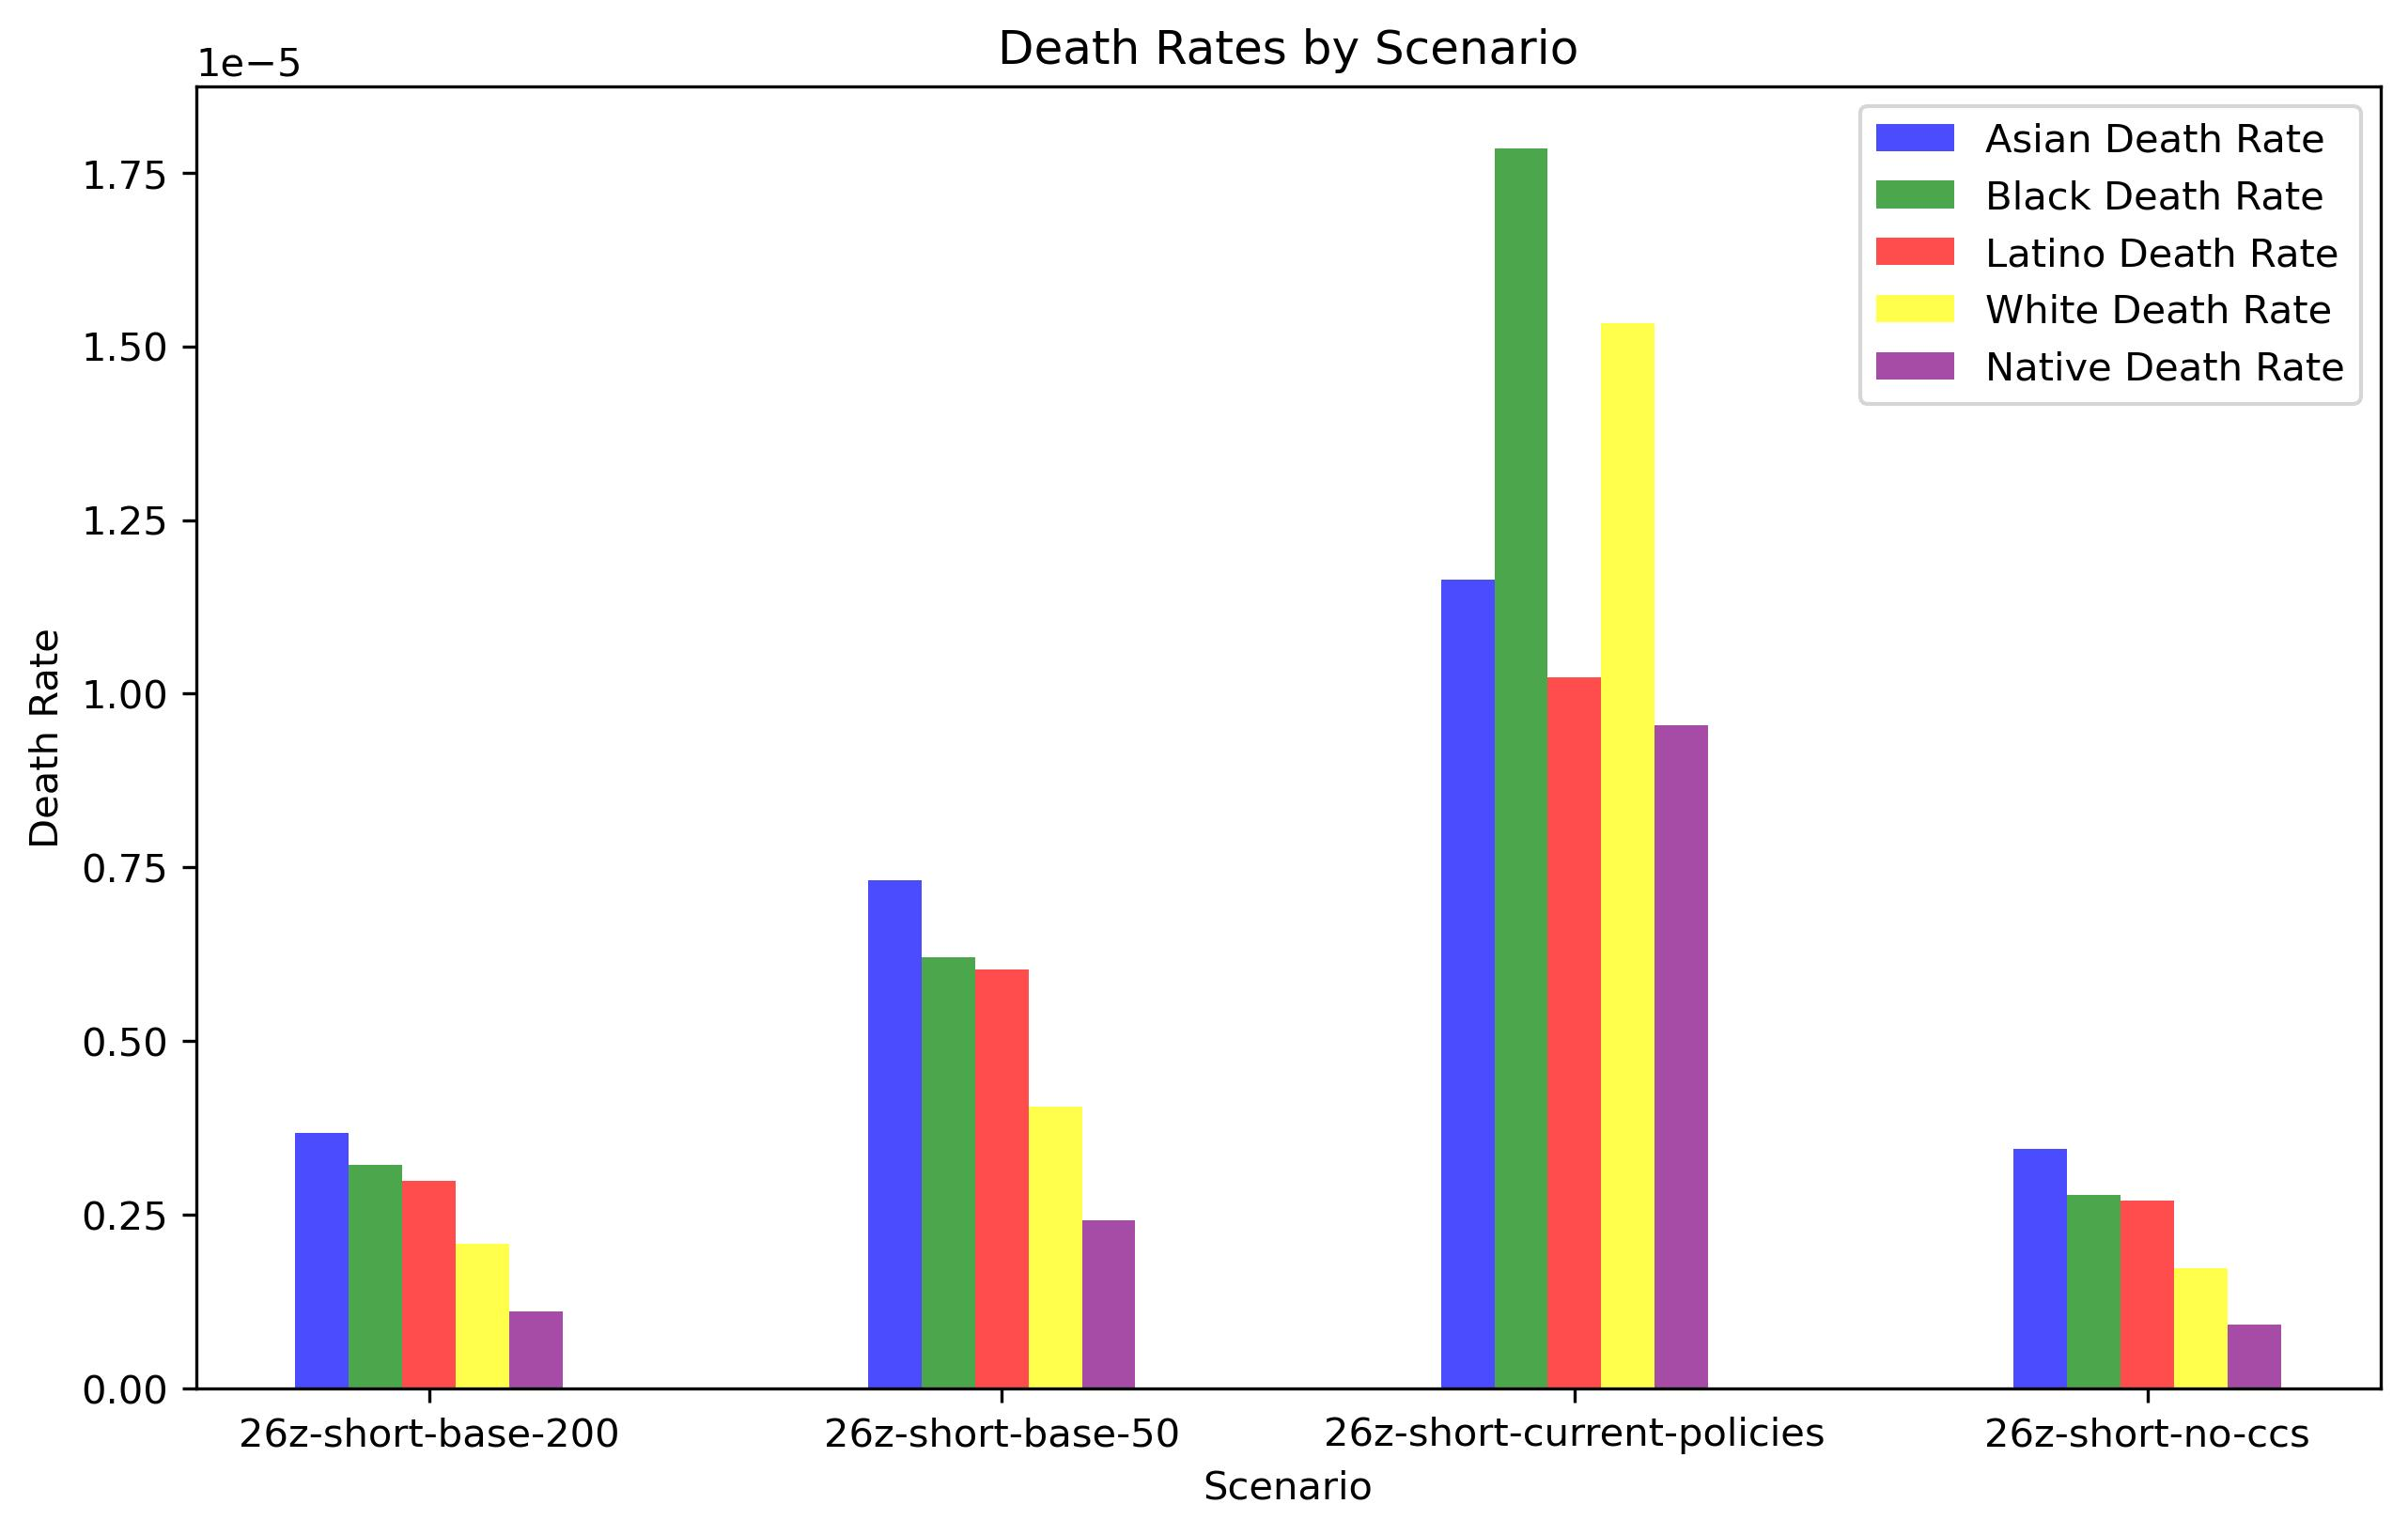
\includegraphics[width=0.3\textwidth]{Figures/Output/ISRM_deathrate_by_scenario_2030.jpg}
    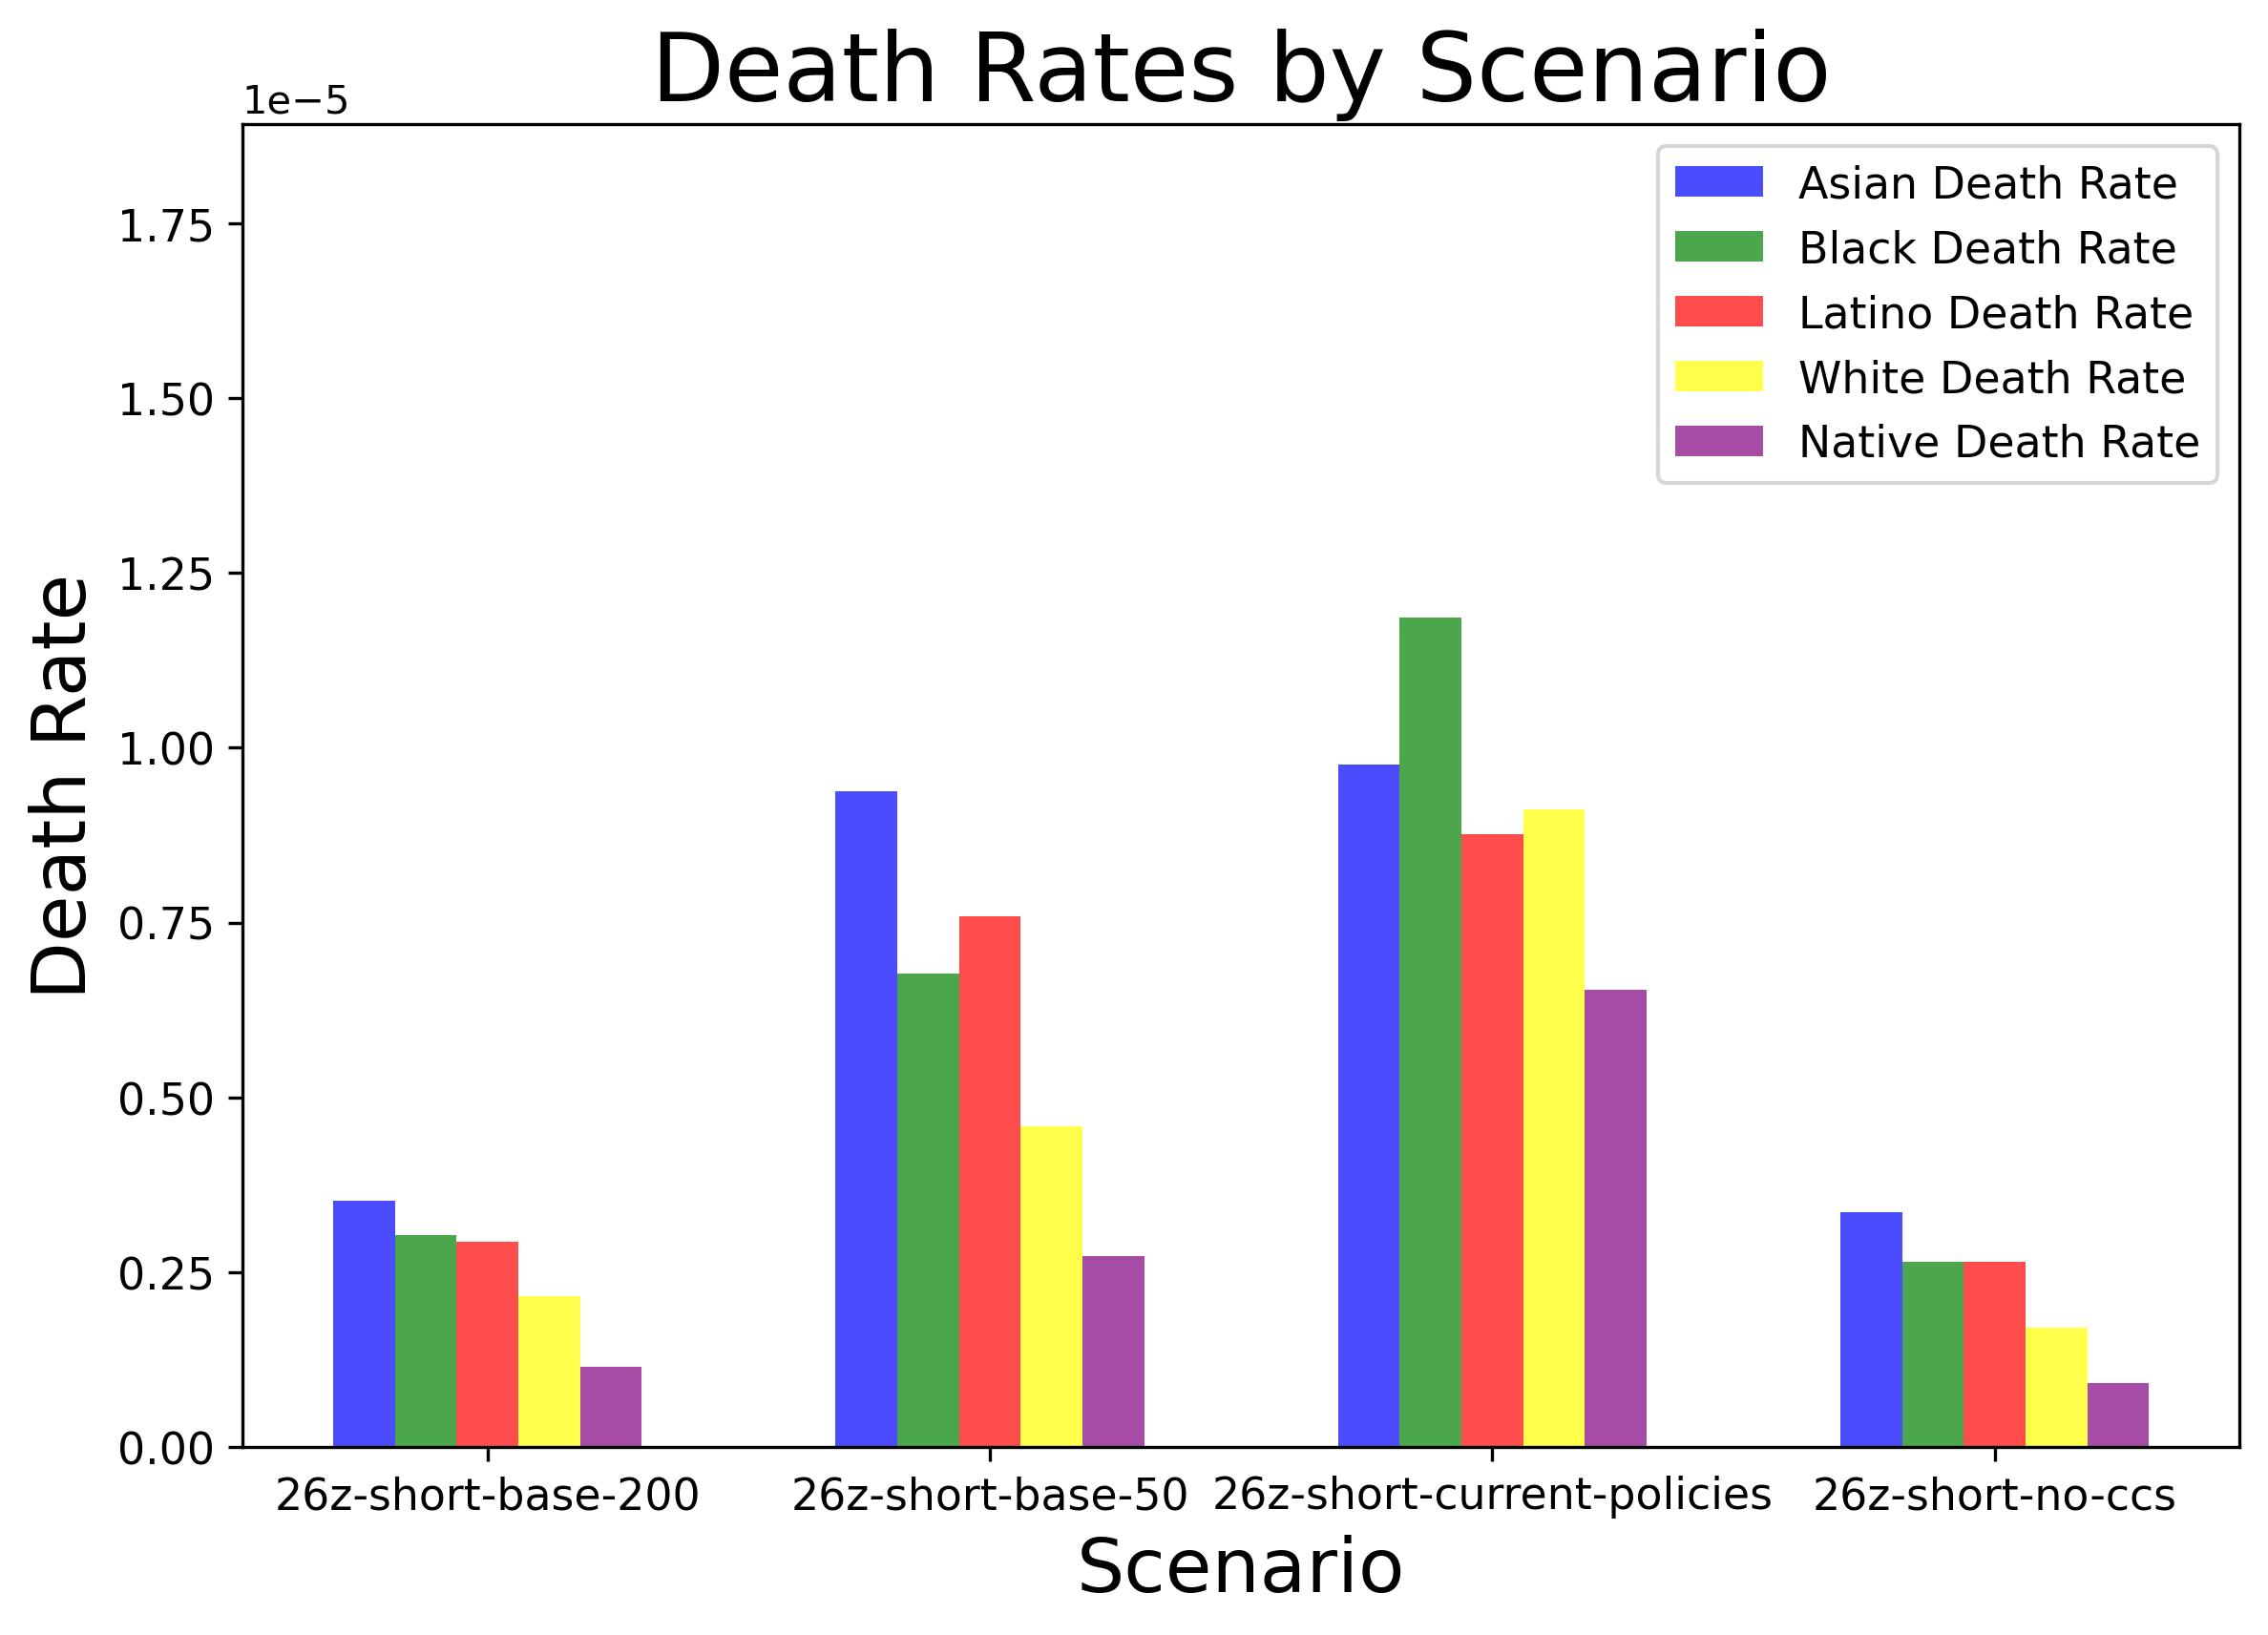
\includegraphics[width=0.3\textwidth]{Figures/Output/ISRM_deathrate_by_scenario_2040.jpg}
    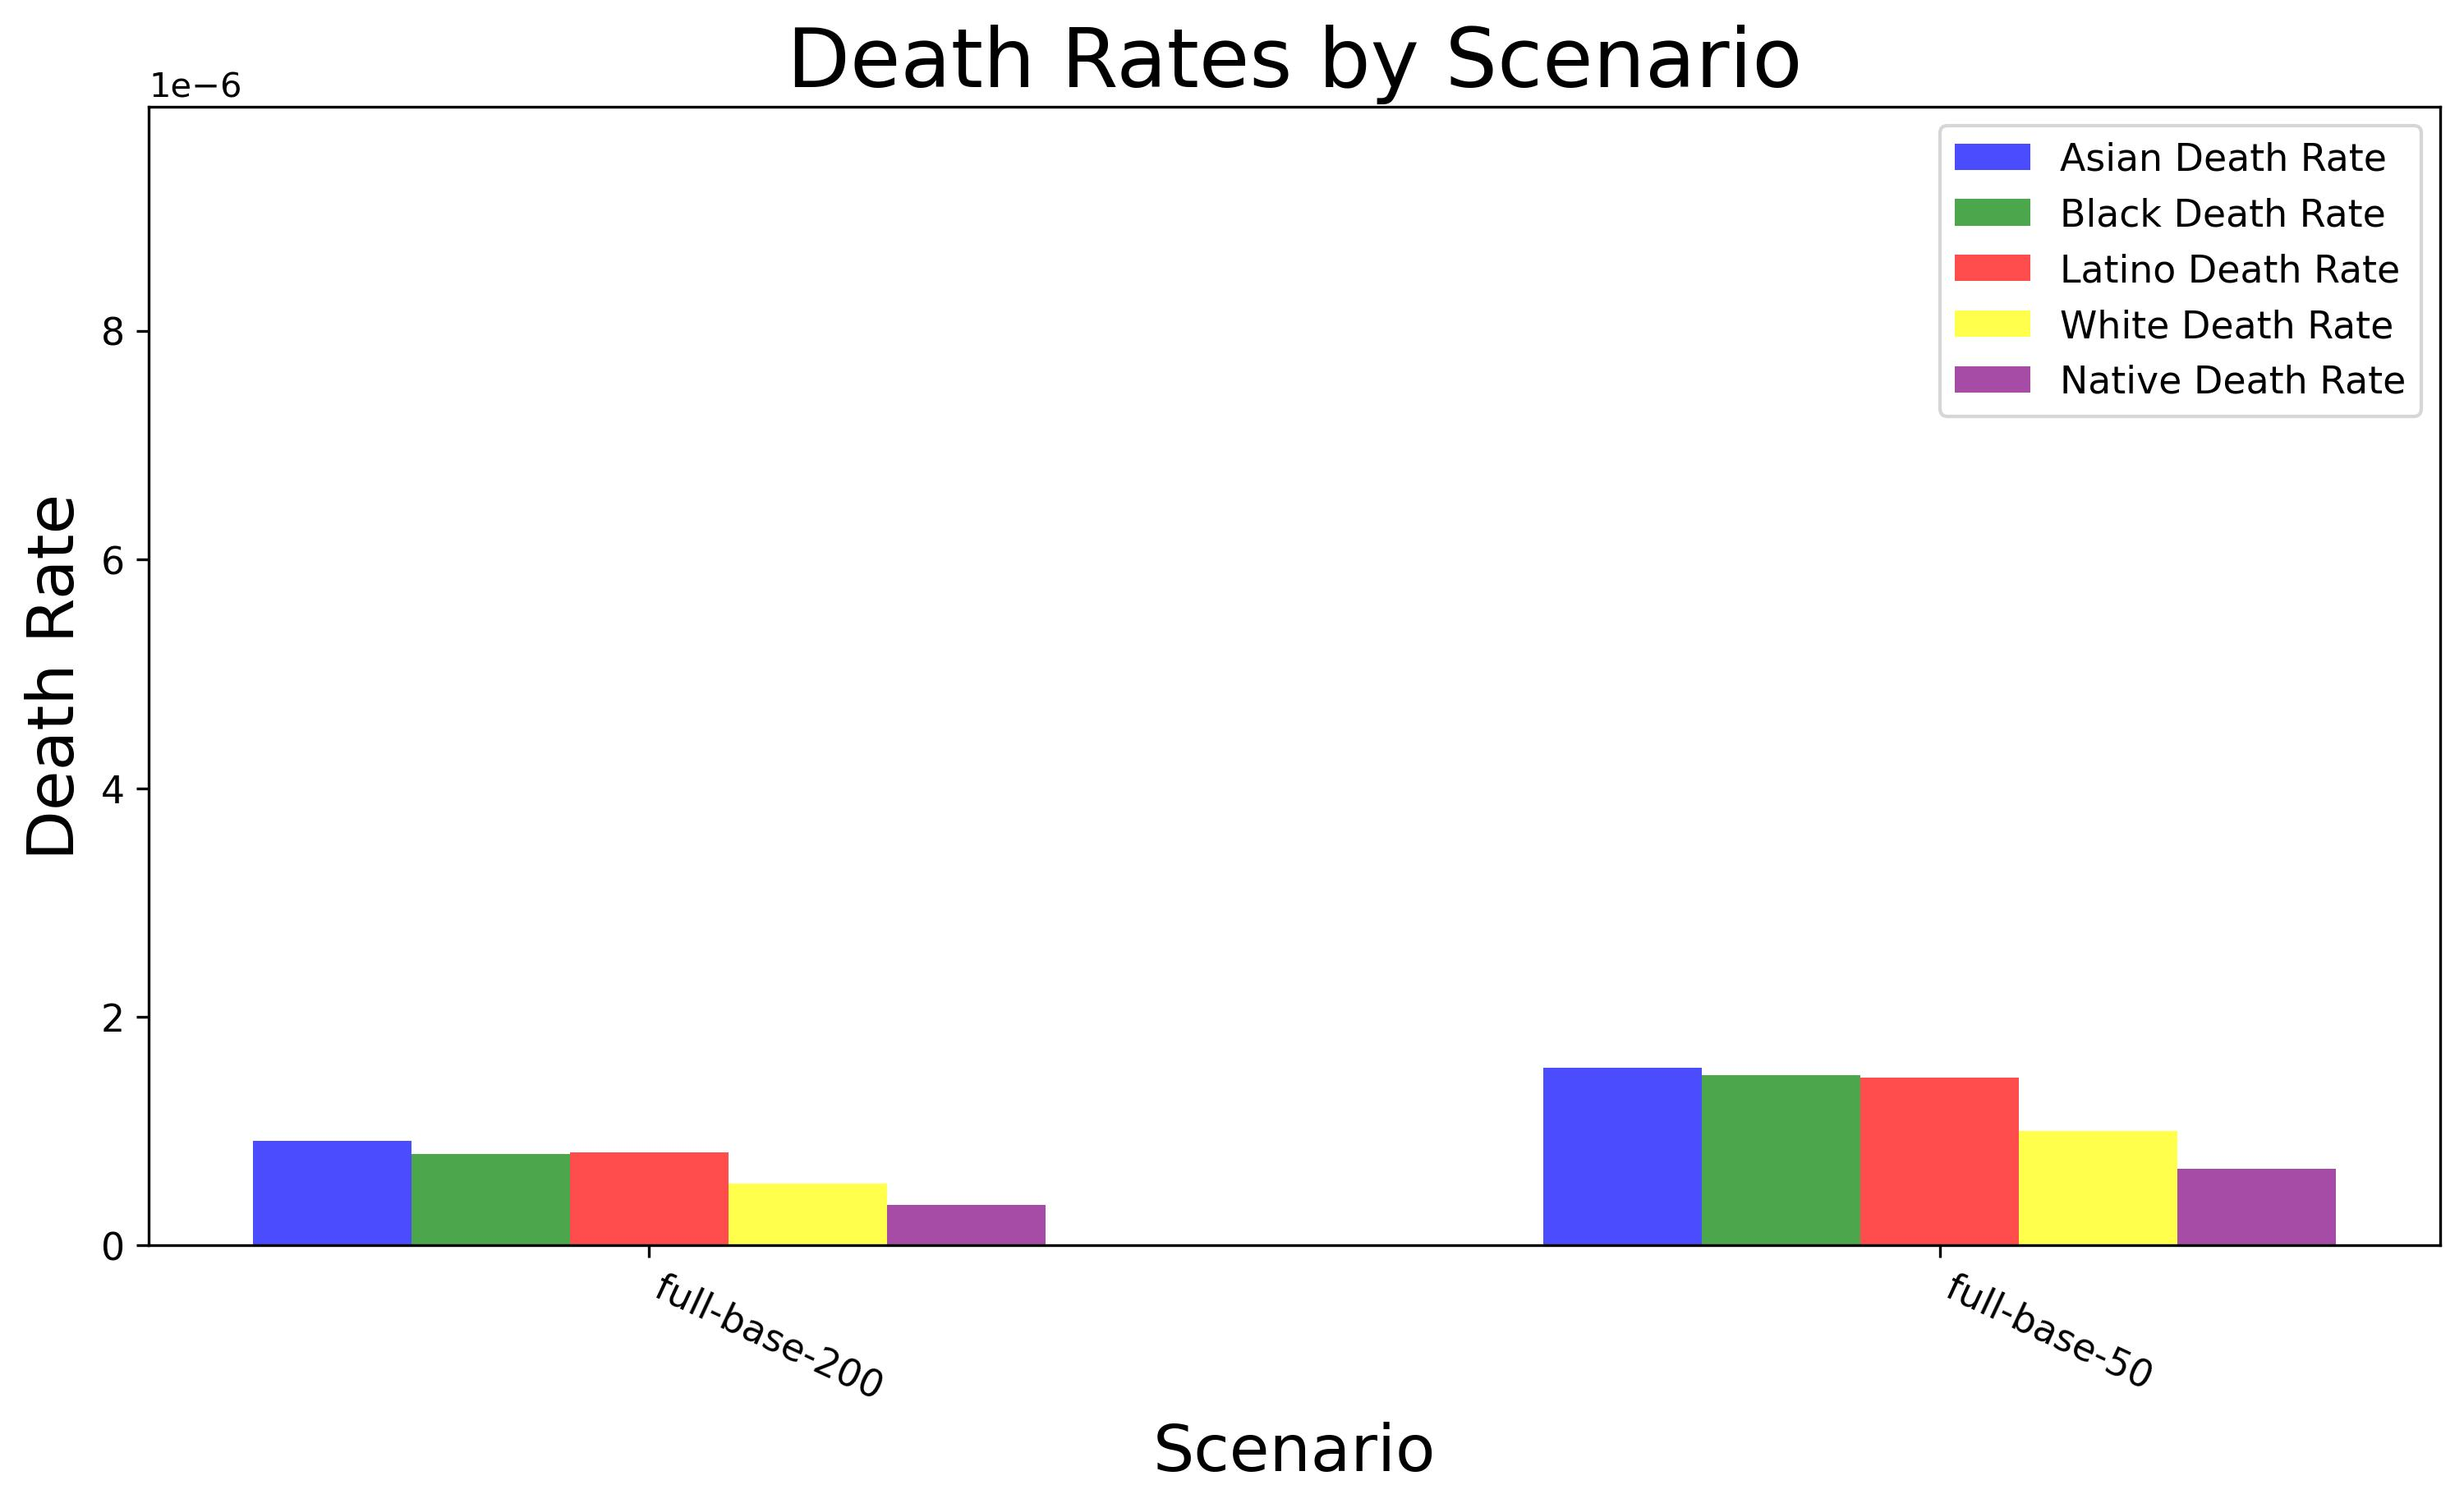
\includegraphics[width=0.3\textwidth]{Figures/Output/ISRM_deathrate_by_scenario_2050.jpg}

\begin{itemize}
    \item Death rates vary widely across racial groups.
    \item Aggressive carbon policies reduce pollution exposure the fastest.
    \item Optimistic -- even under current policies future generations should have much better air quality.
\end{itemize}

\end{frame}

\end{document}